\documentclass[11pt]{book} 
\usepackage{graphicx}
             % Book class in 11 points
\parindent0pt  \parskip10pt             % make block paragraphs
\raggedright                            % do not right justify

\title{\bf Open Calculus}    % Supply information
\author{Editor-in-chief: Adam Cross}   
          %   for the title page.
\date{\today}                           %   Use current date. 

% Note that book class by default is formatted to be printed back-to-back.
\begin{document}                        % End of preamble, start of text.
\frontmatter                            % only in book class (roman page #s)
\maketitle                              % Print title page.


\pagestyle{empty}
%% copyrightpage
\begingroup
\footnotesize
\parindent 0pt
\parskip \baselineskip

This work is subject to the GNU Free Documentation License (version 1.3) with the following additional clause: none of the major publishing houses may distribute this work commercially.

Complete license information is available at smartifybooks.com.

In particular, you may freely copy this work and you may distribute it for free or commercially (except major publishers), and you may edit this work to create your own fork of the project, but any such fork is subject to the same license.  


\vfill

Smartify Books, \\
Baton Rouge, LA \\
\texttt{smartifybooks.com}

%%%%{\LARGE\plogo}
\vspace*{2\baselineskip}


\endgroup
\clearpage








\tableofcontents                        % Print table of contents








\mainmatter                             % only in book class (arabic page #s)

\part{A Part Heading}                   % Print a "part" heading



\chapter{Limits}     


\section{Exercises}

\begin{enumerate}

\item
Refer to the graphs.

\begin{center}
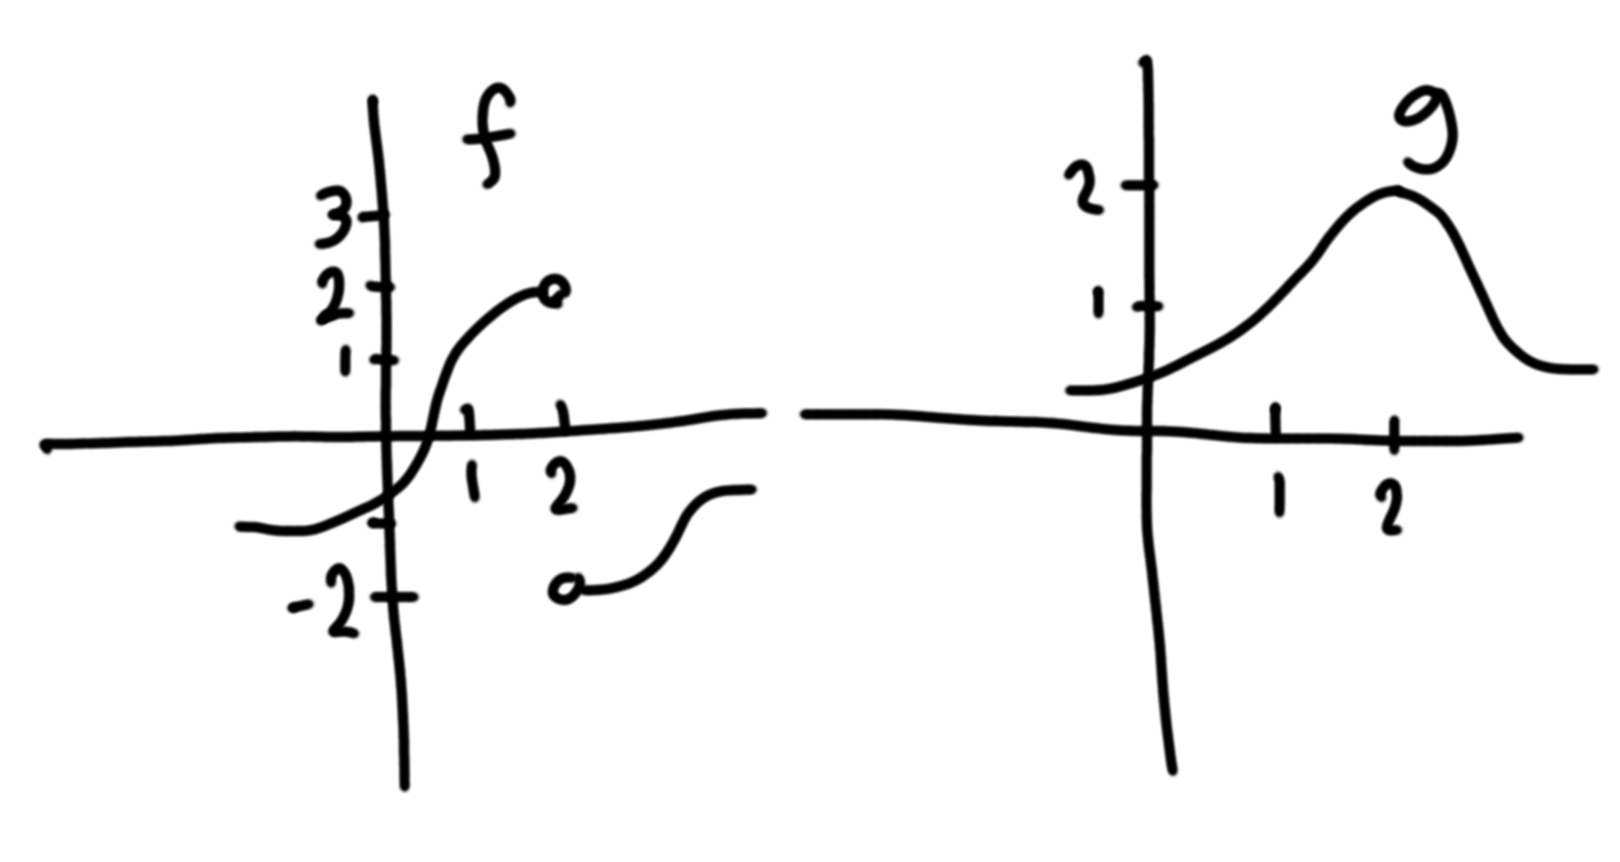
\includegraphics[width=4in]{limitExerciseImage1.png}
\end{center}

What is $\lim_{x\to 2} f(g(x))$?  What is $\lim_{x\to 2} g(f(x))$?




\item 

We will consider the limit $$\lim_{x\to 0} x^3.$$ 

\begin{enumerate}
\item 
Sketch a graph of $x^3$ around x=0 and draw two horizontal lines representing $\epsilon$ and $-\epsilon$. 



\item \label{b}
 What is the largest (most positive) value x can be so that   $x^3\leq \epsilon$?  
 

 
 \item \label{c}
  What is the most negative value x can be so that $x^3\geq -\epsilon$?



\item
What $\delta$ should we choose so that when $|x-0|<\delta$ we can be sure that $|x^3-0|<\epsilon$?  (Here we write the ``- 0'' part for emphasis so that it looks like the definition of a limit, but it can (and should) be omitted in most writing.  We want $\delta$ small so that $(x-\delta,x+\delta)$ is in the interval you identified in parts \ref{b} and \ref{c} above.



\item
If we require $|x^3-0|<1/1000$, how small does $|x|$ have to be?  



\end{enumerate}

\item

Explain in simple terms why $$\lim_{x\to 0} \frac{1}{x}$$ does not exist.  



\item
Explain in words why $$\lim_{x\to 0} x^2 \sin(2\pi/x)=0$$ (meaning the limit exists and is 0) but the limit $$\lim_{x\to 0} \sin(2\pi/x)$$ does not exist.  You are not required to write a proof, but explain what the essential difference is.









\end{enumerate}




\chapter{Derivatives}  


\section{Practice Quiz}

For the best learning experience, treat a practice quiz like an in-class quiz. Don't refer to other parts of the textbook.

\begin{enumerate}


\item Circle T for true or F for false:
\begin{enumerate}
\item T/F For any numbers $a$ and $b$, where $a<b$, there is a rational number $p/q$ so that $a<p/q<b$.

\item T/F The number $\sqrt{2}$ can be written as $p/q$ where $p$ and $q$ are both integers.

\item T/F The limit $\lim_{n\to \infty} (1+1/n)^{n}$ does not exist.

\item T/F It's possible to find a rational number as close to $\pi$ as you want.

\end{enumerate}


\item Compute the derivative.  

\begin{enumerate}
\item
$\frac{d}{dx} e^{\sin(x)}$
\item
$\frac{d}{dx} \ln(\cos(x))$
\item
$\frac{d}{dx} x^3\tan(x)$
\item
$\frac{d}{dx} \sin(x)^x$
\end{enumerate}




\item
Compute the derivative $\frac{d}{dx} \sin^{-1}(x)$ using the chain rule/implicit differentiation technique.  



\item Let's think about how to approximate $\sin(1^\circ)$.

\begin{enumerate}


\item  Since $1^\circ$ is close to $0^\circ$, we will find a tangent line at 0.  But why is $0^\circ$ any easier than $1^\circ$?



\item What is the slope of the tangent line at $0$?



\item What is the equation of the tangent line at $0$?



\item What is the value of the tangent line at $1^\circ$?  (Be sure to convert into radians.)



\item Why is your answer in the previous part a reasonable approximation to $\sin(1^\circ)$?

\end{enumerate}


\end{enumerate}





\chapter{Integrals}  



\end{document}                         